\section{Smooth 0--1 Loss Approximation}
\label{cha:Smoothlossapprox}

The non-smooth, non-differentiable 0--1 loss can be
approximated by a smooth, differential sigmoidal loss as follows:
$$l_i = \mathbb{I} [t_i \w^T \xi \leq 0] \approx \frac{1}{1 + e^{Kt_i \w^T \xi }}.$$
This approximation is illustrated by Figure \ref{fig:sla.smooth} (top) for different
values of the \emph{precision constant} $K \in \R^+$ that modulates smoothness.
Assuming the $\xi$ do not lie
directly on the decision hyperplane, then 
$$\lim_{K \rightarrow +\infty} \frac{1}{1 + e^{Kt_i \w^T \xi }} = l_i.$$

%%%%%%%%%%%%%%%%%%%%%%%%%%%%%%%%%%%%%%%%%%%%%%%%%%%%%%%%%%
\begin{figure}[tp!]
\hspace{-3mm} 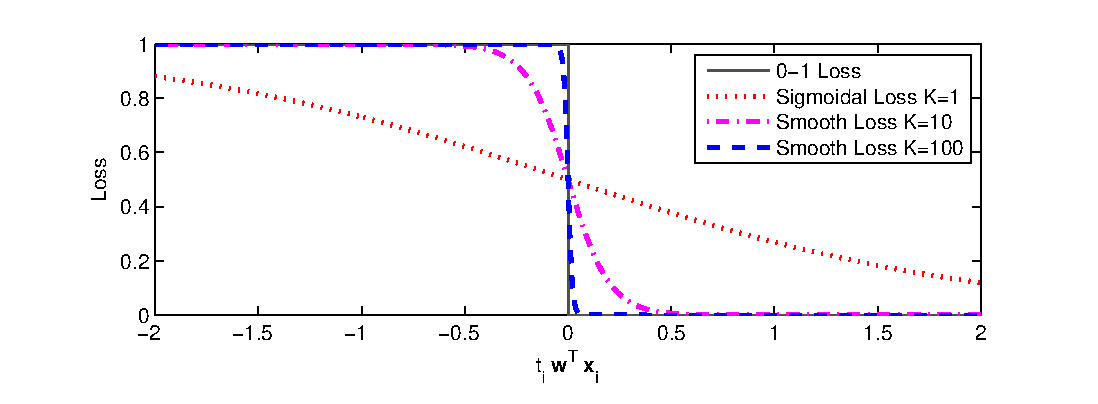
\includegraphics[width=0.50\textwidth]{images/fig52_smooth.eps}
\vspace{-4mm} \hspace{-3mm} 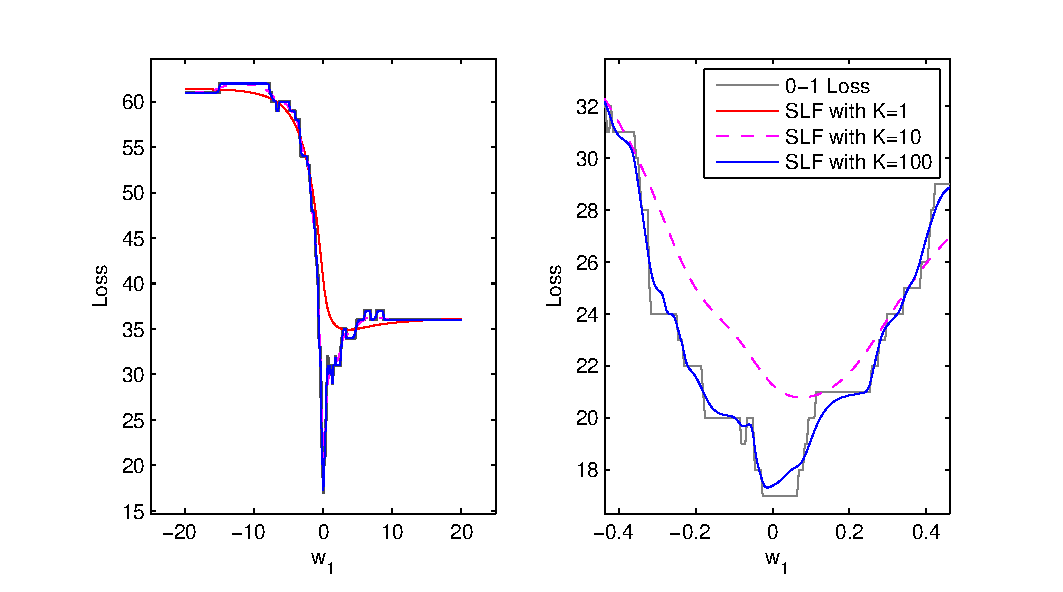
\includegraphics[width=0.50\textwidth]{images/fig53_smoothfunction.eps}
\vspace{-1mm}
\caption{ \footnotesize (top) Sigmoid approximation of 0--1 loss for varying
  $K$.  (bottom) Smoothness of the 0--1 loss for synthetic data vs. $w_1$ with
  other components of $\w$ held fixed.  The plot on the right is a
  close-up of the plot on the left around the global minimum.}
\label{fig:sla.smooth}
\vspace{-1mm}
\end{figure}
%%%%%%%%%%%%%%%%%%%%%%%%%%%%%%%%%%%%%%%%%%%%%%%%%%%%%%%%%%

Figure
\ref{fig:sla.smooth} (bottom) illustrates how this smooth loss
function changes with different values of the precision constant $K$.
Clearly, small $K$ yield smooth losses with few local minima but
provide a rough approximation while large $K$ approach the true 0--1
loss with many local minima.

This suggests the following iteratively unrelaxed optimization approach
for zeroing in on the optimum 0--1 loss value:
\begin{description}
\setlength{\itemsep}{0cm}
\setlength{\parskip}{0cm}
\item[Step 1:] \hfill \\ Find the optimal solution, $\w^*$, of the
  smooth loss function corresponding to a small value of $K$ (e.g.,
  $K=1$) in a wider range (radius) around some initially approximated
  value of $\w$.
\item[Step 2:] \hfill \\ Use the previously found optimal solution as
  the initial approximation to start the search for the new minimum of
  the smooth loss function corresponding to an increased precision
  constant $K$ (e.g., K=10, 100, \dots) and reduced search radius
  (e.g., by a half). This step is repeated again and again until a
  desired level of the precision has been reached (e.g., $K=1000$).
\item[Step 3:] \hfill \\ The last optimal solution, $\w^*$, found in
  Step 2, which is the one corresponding to the desired level of
  precision, is returned as the approximation to the optimal solution
  of 0--1 loss.
\end{description}

This is, of course, just a very rough idea and many things need to be
clarified. The most important thing is perhaps the range optimization
process: given a precision constant $K$, a radius $R$, an initial
guess $\w$, how to efficiently find the optimal solution, $\w^*$, of
the corresponding smooth loss function?

All steps in the sketch of the smooth loss approximation algorithm
given in the previous section repeatedly rely on a range optimization
process, which is described as follows. Given a radius $R$, a
precision constant $K$, and an initial value of $\w$, find the minimum
of the smooth loss function evaluated with the given value of $K$ in
the given radius $R$ around the given initial approximation $\w$. This
subsection, therefore, aims at providing an algorithm tailored for
this task.

Finding the exact minimum in the given range is hard.  Therefore, a
specialized approximation algorithm is being proposed for the range
optimization process. The proposing algorithm is a mixture of the
gradient descent method \cite{Cauchy}, the pattern search method
\cite{Hooke}, and the hill climbing heuristic. It, thus, possesses
advantages of all these methods. This algorithm is detailed in
Algorithm \ref{alg:sla.range}, and a step by step description is being
given next.

%%%%%%%%%%%%%%%%%%%%%%%%%%%%%%%%%%%%%%%%%%%%%%%%%%%%%%%%%%%%%%%%%%%%%%
\begin{figure}[tp!]
\vspace{-3mm}
\caption{\footnotesize
Range Optimization for SLA.\hfill\;\\
\text{\hspace{1.4cm}} $Input$: $\w$, $K$, radius $R$, step size $\epsilon_S$. \\
\text{\hspace{1.4cm}} $Output$: Approx. optimal solution $\w^*$ 
}
\label{alg:sla.range}
{\footnotesize
\begin{algorithmic}[1]
\Function{Grad-Desc-in-Range}{$\w, K, R, \epsilon_S$} 
\Repeat
   \Statex \Comment{{\bf Stage 1}: Find a local minimum \hfill$\qquad\qquad$ \;}
   \State $\w^* \gets \w$
   \Repeat
      \State $r \gets max_{rate}$
      \State $\w \gets (\w^* - r \nabla L_K(\w^*))$
      \While{$(r \!\! \geq \!\! min_{rate}) \!\! \land \!\! (L_K(\!\w^*) \!\! - \!\! L_K(\w) \!\! < \!\! \epsilon_L) $}
         \State $r \gets 0.1 r$
         \State $\w \gets (\w^* - r\nabla L_K(\w^*))$
      \EndWhile
      \If{$r \geq min_{rate}$}
         \State $\w^* \gets \w$
      \EndIf
   \Until{$(-\epsilon_G \preccurlyeq  \nabla L_K(\w^*) \preccurlyeq \epsilon_G) \lor (r < min_{rate})$}
   \Statex \Comment{{\bf Stage 2}: Probe in radius $R$ to escape minimum}
   \For {$i=0$ to $D$}
      \For{$step \! \in \! \{\epsilon_S,\! -\epsilon_S, 2\epsilon_S,\! -2\epsilon_S, \dots, R, \! -R \}$}
         \State $\w \gets \w^*$  
         \State $w_i \gets w_i + step$
         \If{$L_K(\w^*) - L_K(\w) \geq \epsilon_L$}
            \State {\bf go to step 3}
         \EndIf       
      \EndFor
   \EndFor
%   \Statex
\Until{$L_K(\w^*) - L_K(\w) < \epsilon_L$}
\State \Return $\w^*$
\EndFunction
\end{algorithmic}}
\vspace{-4mm}
\end{figure}
%%%%%%%%%%%%%%%%%%%%%%%%%%%%%%%%%%%%%%%%%%%%%%%%%%%%%%%%%%%%%%%%%%%%%%

The following are some important notes to Algorithm
\ref{alg:sla.range}. In the first process, the biggest possible value
of the update rate $r$ is preferred because of two reasons. Firstly,
this would provide a faster convergence and reduce the number of
loops. Secondly, big update rate make big change in $\w$ and would
allow the algorithm to bypass many local optima and valleys, therefore
better adapt to the general trend of the smooth loss function. In the
second process, the probing locations are points distributed evenly
along the axes of each component of $\w^*$, while probing these points
is much faster than probing the whole $D-$dimensional ball centered at
$\w^*$, there are cases when this method fails to detect better
solutions. However, as an approximation, this method works
considerably well in practice. Overall, it can be seen, that whenever
$\w^*$ is updated, its corresponding loss value must be reduced by at
least an amount of $\epsilon_L$. Thus, the returned solution $\w^*$ is
guaranteed to be at least as good as the initial approximation $\w$,
which was given as input. This range optimization algorithm will be a
major component of the SLA algorithm being introduced in the next
subsection.

The Smooth Loss Approximation (SLA) algorithm in
Figure~\ref{alg:sla.algorithm} represents a detailed SLA algorithm,
the step by step explanation of which is being given next.

%%%%%%%%%%%%%%%%%%%%%%%%%%%%%%%%%%%%%%%%%%%%%%%%%%%%%%%%%%%%%%%%
\begin{figure}
\vspace{-3mm}
\caption{
Smooth 0--1 Loss Approximation (SLA). \\
\text{\hspace{1.4cm}} $Input$: Training data $(\boldsymbol{X},\t)$. \\
\text{\hspace{1.4cm}} $Output$: Weights $\w^*$ minimizing 0--1 loss.
}
\label{alg:sla.algorithm}
{\footnotesize
\begin{algorithmic}[1]
\Function{Find-SLA-Solution}{$\X, \t$} \Comment{returns $\w^*$}
   \State $\w^* \gets \w^*_{\mathit{SVM}}$ from SVM solution for $(\boldsymbol{X},\t)$
   \State $R \gets R0$
   \State $\epsilon_S \gets \epsilon_{S0}$
   \State $K \gets K_{MIN}$
   \While {$K \leq K_{MAX}$}
      \State $\w^* \gets$ \Call{Grad-Desc-in-Range}{$\w^*, K, R, \epsilon_S$}
      \State $K \gets r_K.K$
      \State $R \gets r_R.R$
      \State $\epsilon_S \gets r_\epsilon.\epsilon_S$
   \EndWhile
   \State \Return $\w^*$
\EndFunction
\end{algorithmic}}
\vspace{-4mm}
\end{figure}
%%%%%%%%%%%%%%%%%%%%%%%%%%%%%%%%%%%%%%%%%%%%%%%%%%%%%%%%%%%%%%%%

The input and output of Algorithm \ref{alg:sla.algorithm} is the same
as for all other 0--1 loss optimization algorithms introduced in this
thesis. This algorithm returns $\w^*$ -- an approximated solution of
0--1 loss optimization problem. The description of steps of this
algorithm is as follows. Step 2 initialize $\w^*$ to a weight vector
approximated by a fast classifier, e.g., by linear SVM, as has been
always mentioned so far. Step 3 and 4 initialize the radius $R$ and
the step size $\epsilon_S$ to the values of given constants $R0$ and
$\epsilon_{S0}$. In step 5, the precision constant is initialized to
$1$, and the while loop in steps 6 to 11 ensures that $K$ is increased
gradually until a desired precision level $K_{MAX}$ has been
reached. Step 7 calls the {\sc Grad-Desc-in-Range} function to
optimize $\w^*$ in accordance with parameters $K, R, \epsilon_S$ and
the initial approximation is the current value of $\w^*$. Steps 8, 9,
10 then updates the parameters for the next loop. Specifically, $K$ is
increased to $r_K.K$, where $r_K>1$ is the update rate of
$K$. Similarly, $r_R$ and $r_\epsilon$ are the update rates of $R$ and
$\epsilon_S$. These must be, however, less than 1, because radius and
step size must be reduced in each loop. When the precision constant
$K$ has reached the required level of precision $K_{MAX}$, the loop
terminates, and the value of $\w^*$ is returned as the best
approximation to optimal solution of 0--1 loss optimization problem.

Sensible values for the constants given in Algorithm
\ref{alg:sla.algorithm} are, for example, the followings:
\[ \begin{array} {lll}
& r_R = 2^{-1}, &R0 = 8, \\
& r_\epsilon = 2^{-1}, &\epsilon_{S0} = 0.2, \\
& r_K = 10, &K_{MIN} = 2, \quad K_{MAX} = 200.
\end{array} \] 
In this case the precision constant $K$ will gain values 2, 20, 200 in
this given order. The corresponding values for radius $R$ are 8, 4, 2,
and for the step size $\epsilon_S$ are 0.2, 0.1, 0.05. This setting
seems to work well in practice for both data normalized to zero mean
unit variance or squeezed into the $[0,1]$ range. This also works
reasonably good for unnormalized data in many cases. In fact, this
setting is used in all tests in this thesis where SLA algorithm is
used, therefore it is verified by the good performance of SLA in those
tests. For instance, Figure \ref{fig:sla.approxsumm} and Figure
\ref{fig:sla.approxlosses} provides visual result of tests that
compare the accuracy of the two approximation algorithms proposed in
this thesis: the combinatorial search approximation (CSA) and SLA. The
results shown in these figures are from 30 synthetic datasets of size
$N=80$ and $D=3$. Also shown in these figures are optimal results
given by running the prioritized combinatorial search as a
reference. It can be seen from these figures, that CSA and SLA have
very similar approximation accuracy, and both are quite close to the
optimal solution.
